%\documentclass[12pt, letterpaper]{article}
\documentclass[a4paper,onecolumn,twoside]{article}
\usepackage[utf8]{inputenc}
\usepackage{comment}
\usepackage[top=2.54cm, bottom=2.54cm, left=2.54cm, right=2.54cm]{geometry}
\usepackage{graphicx}
\usepackage{CJK}
\renewcommand\thepage{}
\newcommand{\sihao}{\fontsize{14pt}{\baselineskip}\selectfont}
\newcommand{\wuhao}{\fontsize{10.5pt}{\baselineskip}\selectfont}
\newcommand{\xiaosihao}{\fontsize{12pt}{\baselineskip}\selectfont}
\newcommand{\xiaoerhao}{\fontsize{18pt}{\baselineskip}\selectfont}
\newcommand{\yihao}{\fontsize{28pt}{\baselineskip}\selectfont}
\newcommand{\sanhao}{\fontsize{15.75pt}{\baselineskip}\selectfont}

% Title EXPERIMENTAL REPORT
\title{EXPERIMENTAL REPORT}
\author{CHENG Zihua}
\date{2019/10/7}

\begin{document}
\begin{CJK*}{GBK}{song}{\wuhao}
\begin{titlepage}
\maketitle
\end{titlepage}

%\tableofcontents
\clearpage



\begin{abstract}
The information on the SAR image is the reflection of the ground object on the radar beam, mainly the image information formed by the backscattering of the object. Here we mainly do two tasks. First, we use the SAR image to select the urban area, obtain the gray image histogram through MATLAB, so perform equalization to obtain the equalized image and histogram, and perform Gaussian fitting on the histogram. On the other hand, the urban area is directly selected from the HH channel data of the SAR image and a histogram is obtained, and the histogram is exponentially fitted based on the maximum likelihood estimation.
\end{abstract}
\noindent%ժҪ������
\begin{flushleft}
\noindent
\qquad Keywords: Image processing, Histogram, Function fitting
\end{flushleft}
\clearpage

\begin{flushleft}
\noindent{\CJKfamily{song}\sanhao\bf 1 Related theory of SAR images}
\end{flushleft}
\begin{flushleft}
\noindent{\CJKfamily{song}\sihao\bf 1.1 Histogram equalization}
\end{flushleft}

\begin{flushleft}
Image enhancement is the use of image enhancement techniques for the overall or local features of a digital image to make the important information of the image more visible. Converting a histogram to a uniformly distributed histogram is the basic idea of the histogram equalization method, which increases the dynamic range of the original pixel gray value.
\end{flushleft}

\begin{flushleft}
\qquad The histogram equalization of the image is a discrete form. The number of pixels of a pair of images is n, there are l gray levels, and n{\tiny k} represents the number of pixels with a gray level of r{\tiny k}, then the kth gray level appears. Probability can be given by\\
\begin{figure}[ht]

\centering
\includegraphics[scale=0.3]{E:/Statistics-SAR/image/1-1.png}
\label{fig1}

\end{figure}
\qquad The transformation function a is
\begin{figure}[ht]

\centering
\includegraphics[scale=0.3]{E:/Statistics-SAR/image/1-2.png}
\label{fig2}

\end{figure}


\qquad The gray value of the equalized pixel can be directly calculated from the histogram of the original image.
\end{flushleft}

\begin{flushleft}
\noindent{\CJKfamily{song}\sihao\bf 1.2 Maximum likelihood estimation}
\end{flushleft}

\begin{flushleft}
The principle of likelihood was formalized by R. A. Fisher. In most
practical situations it produces unique estimators, and has good
and well-known properties. It should be used whenever possible.
\qquad Consider again the sample independent of random variables X={X{\tiny 1},X{\tiny 2},...,X{\tiny n}} each with the same distribution characterized(without lack of generality) by the density f(X{\tiny i};��).The likelihood function is

\begin{figure}[ht]

\centering
\includegraphics[scale=0.4]{E:/Statistics-SAR/image/1-3.png}
\label{fig3}

\end{figure}
Notice that L is not a joint density function, as it depends on �� , not
on the variables.\\
\qquad The principle of maximum likelihood proposes as estimator for ��
the parameter that maximizes.It is given by\\
\vspace{5mm}
\begin{flushleft}
\centering ��=argmax{L(��;X)}\\
 \vspace{5mm}
\end{flushleft}
the point in �� that makes the observations most plausible. It
sometimes coincides with some analogy estimators.
\end{flushleft}

\clearpage
\begin{flushleft}
\noindent{\CJKfamily{song}\sanhao\bf 2 Experiment}
\end{flushleft}
\begin{flushleft}
\noindent{\CJKfamily{song}\sihao\bf 2.1 SAR image data}
\end{flushleft}

\begin{flushleft}
Synthetic Aperture Radar (SAR) emits electromagnetic pulses and records the signals returned from the target. It operates in the microwave region of different frequency bands. Frequency and other parameters (such as angle of incidence, polarization, and imaging mode) affect the ability of the sensor to retrieve information from the target. We will start with a complex scattering vector and then reach an exponential distribution to derive the basic properties of the SAR data.

\begin{figure}[ht]

\centering
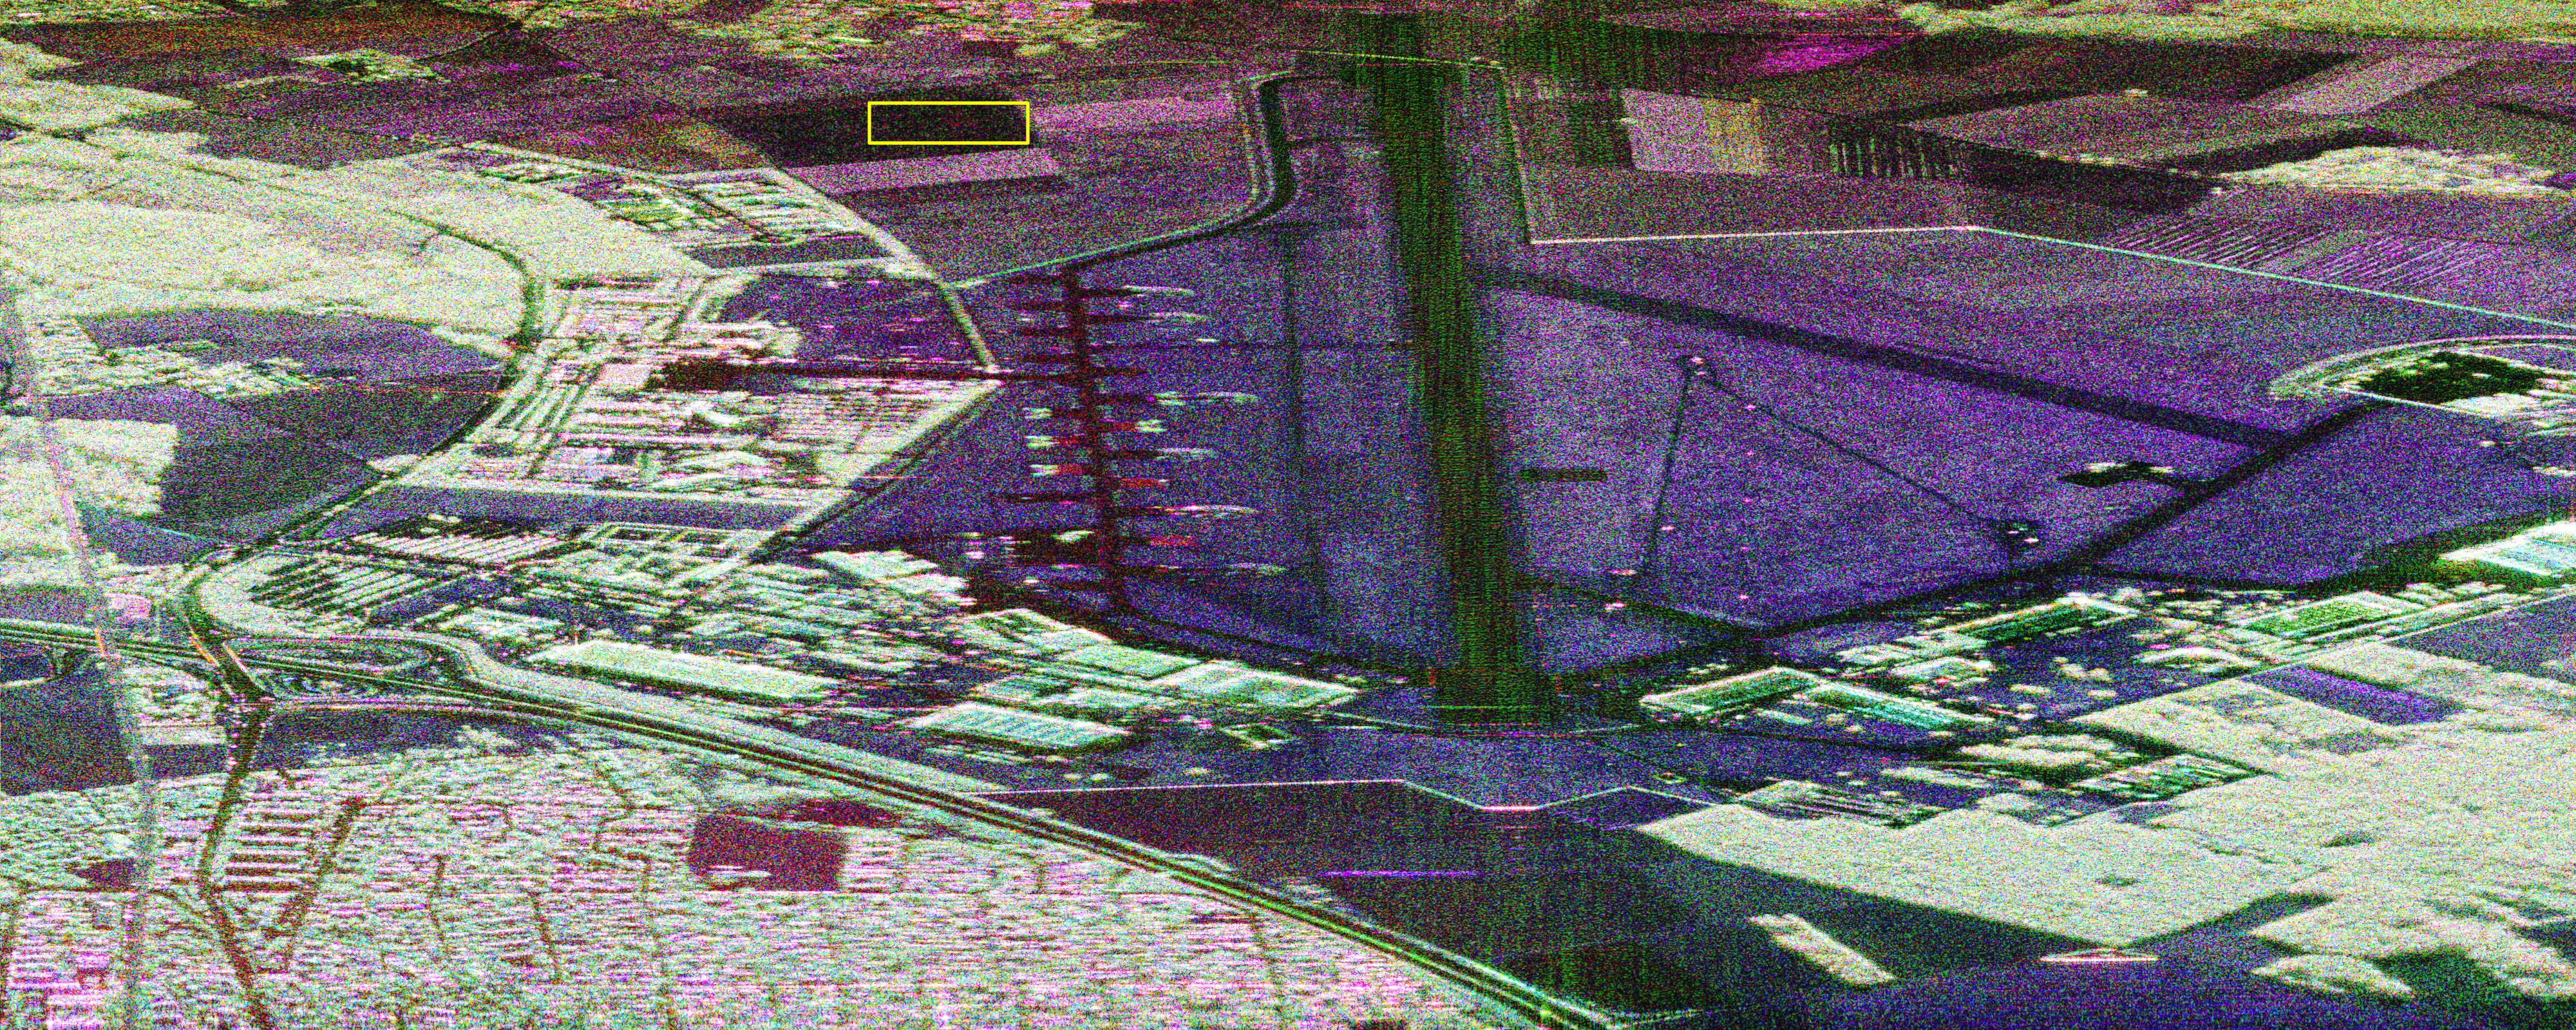
\includegraphics[scale=0.1]{E:/Statistics-SAR/image/2-1.png}
\label{fig1}

\end{figure}

\end{flushleft}

\begin{flushleft}
\centering Figure1:SAR image\\
\end{flushleft}
\begin{flushleft}
\qquad The image has 1599��4000 pixels, and we extract a small piece of urban area at the bottom left for analysis.
\end{flushleft}

\begin{flushleft}
\noindent{\CJKfamily{song}\sihao\bf 2.2 Intercepted town area image}
\end{flushleft}
\begin{flushleft}
According to the sar image, the town area is intercepted by matlab, and the area is equalized. Finally, the histograms of the two images are obtained and fitted.
\begin{figure}[ht]

\centering
\includegraphics[scale=0.3]{E:/Statistics-SAR/image/2-2.png}
\label{fig2}

\end{figure}
\end{flushleft}
\begin{flushleft}
\centering Figure2:Intercepted urban area\\
\end{flushleft}
\clearpage
\begin{flushleft}
We perform gray value processing on the original image to obtain a grayscale image, and further obtain a histogram of the image.
\begin{figure}[ht]

\centering
\includegraphics[scale=0.4]{E:/Statistics-SAR/image/2-3.png}
\label{fig3}

\end{figure}
\end{flushleft}
\begin{flushleft}
\centering Figure3:Grayscale maps and equalized images and histograms of urban areas\\
\end{flushleft}
\begin{flushleft}
It can be seen from the histogram of the gray-scale processed image in Fig. 3 that the data roughly conforms to the Gaussian distribution, so the Gaussian distribution of the data can be fitted according to the maximum likelihood estimation, and the fitting distribution is obtained as shown in Fig4.
\begin{figure}[ht]

\centering
\includegraphics[scale=0.4]{E:/Statistics-SAR/image/2-4.png}
\label{fig3}

\end{figure}
\end{flushleft}

\begin{flushleft}
\centering Figure4:Gaussian fitting map of SAR image\\
\end{flushleft}
\begin{flushleft}
\qquad mu= 1.704233322237017e+02, sigma = 2.429573148593819e+03
\end{flushleft}

\clearpage
\begin{flushleft}
\noindent{\CJKfamily{song}\sihao\bf 2.3 Histogram of HH channel data of SAR image and data fitting}
\end{flushleft}

\begin{flushleft}
According to the HH channel data of the SAR image, the urban area is intercepted by r language, and then the histogram is obtained and the data is fitted.\\
\qquad We select a small part of the intercepted urban area for analysis.
\end{flushleft}

\begin{flushleft}
\begin{figure}[ht]

\centering
\includegraphics[scale=0.4]{E:/Statistics-SAR/image/2-5.png}
\label{fig5}

\end{figure}
\end{flushleft}
\begin{flushleft}
\centering Figure5:Intercepted urban area\\
\end{flushleft}

\begin{flushleft}
\begin{figure}[ht]

\centering
\includegraphics[scale=0.8]{E:/Statistics-SAR/image/2-6.png}
\label{fig6}

\end{figure}
\end{flushleft}
\begin{flushleft}
\centering Figure6:Histogram of all data and restricted histogram\\
\end{flushleft}

\clearpage
\begin{flushleft}
From Figure 6, we can see that the left side is too meaningless for our research because of too much data, so we can set a threshold for processing. Only the portion smaller than the threshold is selected for data fitting. At the same time, we see that the data is consistent with the characteristics of the exponential distribution, so the data is exponentially fitted using the maximum likelihood estimation.
\end{flushleft}

\begin{flushleft}
\begin{figure}[ht]

\centering
\includegraphics[scale=0.4]{E:/Statistics-SAR/image/2-7.png}
\label{fig6}

\end{figure}
\end{flushleft}
\begin{flushleft}
\centering Figure7:Exponential fitting distribution\\
\end{flushleft}

\begin{flushleft}
\noindent{\CJKfamily{song}\sanhao\bf 3 Summary and analysis}
\end{flushleft}

\begin{flushleft}
The real and imaginary parts of the sum of the scattering vectors and S are independent Gaussian random variables with a mean of zero and a variance of ��2/2; ��2 is often referred to as backscattering. The variance of the complex rate of return S for two targets with different backscatters is only different. In general, instead of dealing with complex scattering S directly, it is better to process its amplitude S or the square of S. Without prejudice, we will choose the latter. If the real and imaginary parts of the complex scattering S are independent zero-mean Gaussian random variables with a zero difference ��2/2, the intensity follows an exponential distribution of the mean ��2.
\end{flushleft}

 \vspace{20mm}
\begin{flushleft}
\noindent{\CJKfamily{song}\sanhao\bf Bibliography}\\
 \vspace{2mm}
\noindent [1]E. S. Almeida, A. C. Medeiros, and A. C. Frery. How good are Matlab,Octave and Scilab for computational modelling? Computational and Applied Mathematics, 31(3):523�C538, 2012. doi:10.1590/S1807-03022012000300005.\\
\noindent [2]Haizhen Zhou,Dengfeng Xiong.Application Research of Histogram Equalization Algorithm in Image Gray Processing[J].Technological innovation and application,2015(32):51-52.\\
\end{flushleft}
% Comments
\begin{comment}
This text won't show up in the compiled pdf
this is just a multi-line comment. Useful
to, for instance, comment out slow-rendering
while working on the draft.
\end{comment}
\end{CJK*}
\end{document}
